\documentclass{article}
\usepackage[utf8]{inputenc}
\usepackage{caption}
\usepackage[margin=1in]{geometry}
\usepackage{graphicx}
\usepackage{pdfpages}
\usepackage{float}
\pdfminorversion=7

\begin{document}
\begin{titlepage}


\centering
\vspace*{2cm}
{\Huge Final Project Document\par}
\vspace{.25cm}
{\LARGE Course Evaluation System\par}
\vspace{1cm}
{\Large Team EVAL\par}
\vspace{.2cm}
{\Large Jovon Craig, Sam Elliott, Robert Judkins, and Stanley Small\par}
\vspace{1cm}
{\Large Client: Dr. Harlan Onsrud\par}
\vspace{1cm}
{\Large December 19, 2018\par}
\vspace{11cm}

University of Maine - Fall of 2018 - COS 397

Instructor: Professor Terry Yoo

\end{titlepage}

\newpage

\begin{center}
{
\includegraphics[scale=.2]{images/team_logo.png}} \\ 	\bigskip
{\LARGE Course Evaluation System } \\ \medskip
{\large Final Project Document } \\ \medskip
\end{center}

\tableofcontents

\newpage

\section{Introduction}

\subsection{Purpose of This Project}

For our capstone project, Team EVAL is creating a Course Evaluation System, a web application designed to be intuitive and versatile for college instructors. This new system, which will be tested first at the University of Maine, allows one to quickly create course evaluation surveys and review their responses. Our goal is to have a fully working evaluation system for use at the end of the Spring 2019 semester. By making and documenting the software, the team will have gained valuable skills in software engineering, programming, and technical writing.

\subsection{Purpose of This Document}

This final project document gives an overview of our course evaluation system, the purpose of it, and why we believe it is useful. We first talk about existing evaluation creation software and how they are not tailored to college instructors and administrators, unlike our system. The next section goes into more detail about the system, discussing its requirements, user interface, and architecture. The last section describes what we will deliver to the client, our progress on creating the system so far and the steps we still need to take to successfully complete the project.

This document is intended for the development team, the product client, and potential users of the system. Team EVAL needs this document to guide the products development. The client, Professor Harlan Onsrud, also needs it to verify that we are designing the system according to his needs. The document helps the software's users by informing them what the system is designed to do and how it specifically helps them with their work.

\subsection{References}

Craig, J., Elliott, S., Judkins, R., \& Small, S. 29 October 2018. \textit{System Requirements Specification.}
\vspace{3mm}\newline
Craig, J., Elliott, S., Judkins, R., \& Small, S. 16 November 2018. \textit{System Design Document.}
\vspace{3mm}\newline
Craig, J., Elliott, S., Judkins, R., \& Small, S. 30 November 2018. \textit{User Interface Design Document.}
\vspace{3mm}\newline
Onsrud, H. ``Example Question Selection Form.'' See Appendix D.
\vspace{3mm}\newline
Onsrud, H. ''Report for Professor: Roy Turner'' See Appendix E.
\vspace{3mm}\newline
LimeSurvey: The online survey tool - open source surveys. (n.d.). Retrieved from

https://www.limesurvey.org/.

\section{Purpose of This System}

\subsection{Our Problem}

In 2015, there were more than 4,600 higher-education institutions in the United States. Virtually all of them offer a breadth of college courses for students to complete and take them through their academic careers. At the end of a course, students typically fill out an evaluation so that teachers know what they are doing right and wrong. Unfortunately, many institutions, such as the University of Maine, are behind in using technology for this task.

The University of Maine has traditionally used Scantron sheets for course evaluation forms. As Team EVAL knows, filling in tiny bubbles with pencil and paper is tedious. It is also hard work for the college administration to use Scantron sheets. They need to scan the forms for every student in every course, and the data then needs to be collected in a form that is readable for instructors. The University of Maine must upgrade to keep with the times and exploit today's technology.

\subsection{Existing Survey Software}

Several software solutions currently exist that allow users to create, modify, and publish surveys. One notable example is LimeSurvey, a free and open-source tool that is operated online. The team acknowledges the immense amount of work put into creating LimeSurvey, with its selection of question types, scalability, visualization features, and other powerful functionality. However, LimeSurvey has always been general-purpose software; it is aimed at multiple types of users who want to make surveys.

College teachers and administrators need to jump through hoops to use a tool like LimeSurvey which are not always easy or intuitive. Their evaluations are highly standardized and they are sent to potentially hundreds of students. LimeSurvey and similar software do not account for these qualities. A college instructor would have to manually input every field, question, and class roll into each evaluation from scratch.  UMaine is using another service, Blue by Explorance, that has the necessary functionality, but it is expensive to use for a university and impossible to use for individuals. These are some of the reasons why our client, Dr. Onsrud, wants us to create an evaluation system better suited to instructors.

\subsection{Our Solution}

Our solution to the above problems is to make our own free and open-source course evaluation system, which has simplicity and ease-of-use in mind. Like existing survey software, our system can too create, modify, and publish surveys. But the differences between our software and existing software are great. With the new system, instructors and administrators can select a survey created previously to use again for a different survey. They can modify the class roll at the same time as they modify their evaluation form. Also, survey results are specially displayed to indicate the current performance of an instructor.

There are several way in which users can interact with our novel course evaluation system. First, they can create a new evaluation survey form with any required fields and questions already listed. They can then edit forms that are unpublished or view forms that have already been published. After publishing a survey, students are periodically reminded to complete it by our system. Finally, users can see results on a select group of college courses for each question in a survey.

\newpage

\section{About This System}

\subsection{System Requirements}

Near the beginning of the project, we met with Professor Onsrud to solicit the system requirements, what the evaluation system must do to function as Dr. Onsrud intends. The System Requirements Specification (SRS) divides the requirements into two categories. The functional requirements specify the major actions a user can perform with the system. They are listed in Table 1 below:

\begin{center}

\begin{tabular}{|p{1.5cm}|p{1.5cm}|p{3.5cm}|p{6cm}|} 
\hline
\textbf{Number} & \textbf{Priority} & \textbf{Name} & \textbf{Description} \\
\hline
1 & 5 & Log in to system & A user logs in with a Google e-mail address and password \\ 
\hline
2 & 5 & Create evaluation & A user creates a new evaluation form for a class \\ 
\hline
3 & 5 & Edit evaluation & A user enters and edits information and questions for an evaluation form \\  
\hline
4 & 5 & Publish evaluation & A user publishes an evaluation form \\
\hline
5 & 5 & View evaluation results & The user reviews a course's or category of courses' results \\ 
\hline
\end{tabular}
\captionof{table}{Functional requirements}
\end{center}

The non-functional requirements state the system's qualities that are irrelevant to how the program behaves. They are listed below in Table 2:

\begin{center}
\begin{tabular}{|p{1.5cm}|p{1.5cm}|p{8cm}|}
\hline
\textbf{Number} & \textbf{Priority} & \textbf{Description} \\
\hline
1 & 3 & The software should be supported by the latest versions of Windows, Mac, Linux, iOS, and Android.\\ 
\hline
2 & 4 & The software should be accessible by the latest versions of Safari, Chrome, Firefox, and Edge.\\ 
\hline
3 & 5 & All questions entered by the teacher or administrator shall appear on the output survey.\\  
\hline
4 & 5 & All data stored in the program's database shall be valid.\\
\hline
5 & 5 & All collected survey data shall not be alterable.\\ 
\hline
6 & 4 & Teachers shall not be able to access data of courses other than their own.\\ 
\hline
7 & 3 & The mean time between failures should be at least 60 minutes.\\ 
\hline
8 & 5 & Students shall have no access to any data stored by the program.\\ 
\hline
9 & 5 & All survey responses (except signed \newline comments) shall be anonymous.\\ 
\hline
10 & 2 & The software should scale to at least three universites, 1000 courses per semester, 1000 teachers per university, and 500 students per course.\\  
\hline
11 & 1 & The software should not exceed 500 MB in size.\\
\hline
12 & 4 & The software's source code shall be open-source and shall use a GPLv2 license.\\ 
\hline
13 & 4 & The licensing requirements of any non-original code shall be met.\\ 
\hline
14 & 4 & The software shall meet UMaine AFUM requirements.\\ 
\hline
\end{tabular}
\captionof{table}{Non-functional requirements}
\end{center}

\subsection{System Architecture}

\begin{center}
\begin{figure}[H]
\centering
\vspace{2mm}
\label{fig:componentdiagram}
{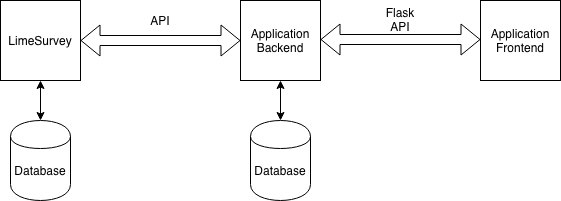
\includegraphics[scale=.75]{images/component_diagram.png}}
\captionof{figure}{Component diagram of the system}
\end{figure}
\end{center}

Our system features a modular design, with many distinct parts which communicate via an API. The front end implements the user interface, written in JavaScript. The back end communicates with the system's databases and is written in Python. We are using two databases, one maintained by LimeSurvey and another maintained by our system. Additionally, the API will communicate with Google Authentication to authenticate users. The design and implementation of our system can be found in the System Design Document (SDD). The system's components are displayed in Figure 1 above.

By maintaining a modular approach to the design of the system, team members can work independently on individual parts, which will then undergo integration testing. Moreover, by keeping the LimeSurvey codebase separate from our system, we can update LimeSurvery without disrupting other parts of the code. 

\subsection{User Interface}

The user interface is a pivotal part of the user experience and is important for our product. The goal of the system is to make an easy-to-use software that allows users to create course evaluations for their classes on a web application.  Users have no interaction with the back-end architecture and will only see the user interface, so the ease of use relies entirely on the front-end UI.  The exact description of every aspect of our user interface can be found in the User Interface Design Document (UIDD). 

The overarching theme for the user interface is ``less is more''.  The interface will have as few extraneous elements as possible, be as intuitive as possible, and not require a large amount of effort to understand the system.  To this end, all functionality of the product should be accessible from the home page, whose wireframe is shown bellow in Figure 2. 

\begin{center}
\begin{figure}[H]
    \centering
    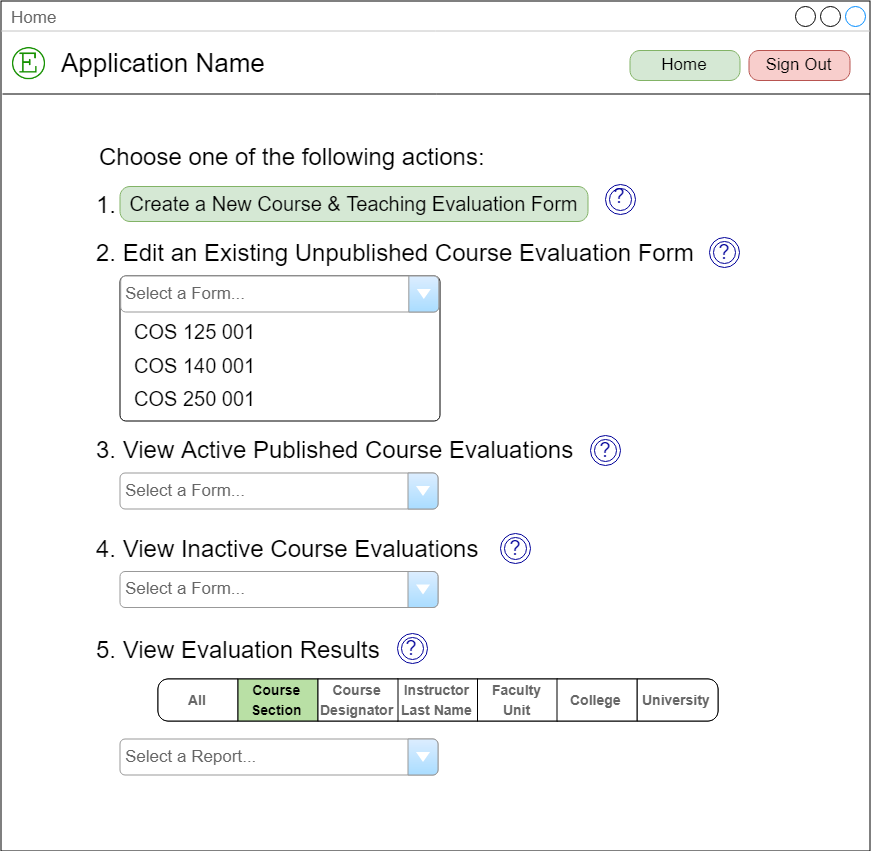
\includegraphics[width=5.5in]{images/home_screen.png}
    \caption{Home screen of the user interface}
\end{figure}
\end{center}

After the landing screen and log-in screen, the user should instantly be aware of the types of functions that one can make through the home screen. To reduce confusion, help text for different features will be present on the same page and not require users to navigate away from it.  The interface will allow users to create new evaluations, view their existing and previous evaluations, and view results of completed evaluations.

\subsection{Tests}

Team EVAL will write several tests in the near future to ensure that the course evaluation system meets all system requirements. These tests are fully described in the system requirements specification. The most important tests concern the overall functionality of the system and integration with LimeSurvey. These will be tested extensively, as they represent the core components of the system. The team will begin testing the non-functional requirements only after all tests for the functional requirements pass.

The team will verify the functional requirements by trying every function available in the course evaluation system. For example, we will create new evaluation forms, edit survey forms, view saved forms, publish forms, and view results for certain courses and categories. Our tests will load mock data into the database so that it is easy to check for correctness. After testing individual functions, we will integrate the components of the system together and run all functional tests at once. Finally, the team will check each non-functional requirement to ensure that the software is acceptable to deliver.

\newpage

\section{Conclusion}

\subsection{Needs This System Meets}

With its high-tech features, our course evaluation system could potentially bring the University of Maine into the modern age. Using our software, an instructor will be able to create a survey with ease, and students will be able to take the whole evaluation form online. The results will automatically be fed back into the software, and the instructor will be able to view statistics of the results and download them afterwards.

This product will eliminate the need for Scantron sheets and provide a fast and simple way to distribute evaluation evaluations to all students in a desired course. The product will be free for use at the University of Maine and by any teachers elsewhere who may be interested in using it.

\subsection{Current Progress}

We have met with our client, Professor Harlan Onsrud, several times over the past few months. Initially we met him to solicit the requirements for the product so that we could deliver something that would both satisfy our customer and potential users of the system. Though it took some time, we eventually came to an agreement, and the requirements were written in detail for us to refer to during development. See the System Requirements Specification for more detail.
	
Next, we started designing our system and the separate components that would be in our implementation, including the front-end user interface, database, API, and how they would interact with the third-party software LimeSurvey. Each component interacts with each other to combine to our final product. Once again, we sat down with our client to discuss the system architecture and he was eventually satisfied with our design. See the System Design Document for more detail.

Once the requirements and architecture were decided, we had to design the user interface of the product. This is arguably the most important part, as this is what the user would be interacting with when using the product. After conferring with our client, we drew up a simple UI that would be easy for the user to use and understand. See the User Interface Design Document for more detail.

The database that will store all our user's class evaluation data is in development. The database schema is finished, and we wrote a script to create it and some mock data. An API is also in development that will help us interface our system with the existing LimeSurvey system. The team has most of the API's endpoints finished, but no tests have been written yet. We have also finished a simple prototype that will allow a user to view all screens of the final product. It is not entirely interactive at the moment, but it gives a glimpse of what the final product may become.

\subsection{Next Steps}

There is still a lot of work to do before our evaluation system is complete. First, the team has to finish implementing all endpoints in the API. We also have to write helper functions that use the LimeSurvey API to publish evaluations and retrieve responses. The user interface prototype needs to be polished to match what our wireframes specify, and the front-end needs functions that interact with the API and the database. Finally, we should include a series of tests for the back end and front end to debug the software and know when we are finished with the system.

The team has several deliverables to send to our client, Dr. Onsrud. So far, we have delivered the system requirements specification, system design document, and user interface design document. In the spring of 2019, we will send a code inspection report, an administrator manual, and a user manual for the evaluation system. Near the end of the school year, we will submit the source code and the final copies of all our documents to Dr. Onsrud electronically. Table 3 lists the date and format that each submission from Team EVAL has been or will be delivered. The dates for incomplete submissions are estimated.
\newpage

\begin{center}
\begin{tabular}{|p{6cm}|p{3cm}|p{3cm}|} 
\hline
\textbf{Submission} & \textbf{Date of Delivery} & \textbf{Format} \\
\hline
System Requirements Specification & 10/29/2018 & Hard Copy\\ 
\hline
System Design Document & 11/16/2018 & Hard Copy\\ 
\hline
User Interface Design Document & 11/30/2018 & Hard Copy\\ 
\hline
Code Inspection Report & March 2019 & Hard Copy\\ 
\hline
Administrator Manual & April 2019 & Hard Copy\\ 
\hline
User Manual & May 2019 & Hard Copy\\ 
\hline
System Requirements Specification & May 2019 & Electronic\\ 
\hline
System Design Document & May 2019 & Electronic\\ 
\hline
User Interface Design Document & May 2019 & Electronic\\ 
\hline
Code Inspection Report & May 2019 & Electronic\\ 
\hline
Administrator Manual & May 2019 & Electronic\\ 
\hline
User Manual & May 2019 & Electronic\\ 
\hline
Source Code & May 2019 & Electronic\\ 
\hline
Web Link to Program & May 2019 & Electronic\\ 
\hline
\end{tabular}
\captionof{table}{List of deliverables to submit}
\end{center}

Next semester, we plan to finish the course evaluation system such that it can be released to the public. In January and February 2019, Stan and Jovon will implement the rest of the API, such as the log-in endpoints and the interaction with LimeSurvey. At the same time, Sam and Robert will work on the front end, perfecting the user interface and writing calls to the API. In March, the team will write and run tests for all system components, with Stan and Jovon on the back end and Sam and Robert on the front end. In April, the whole team will integrate the components and write the integration and system tests. By the final exams in May, the course evaluation system shall be complete and stable, available on http://www.teachingevaluations.org.

\newpage
\section{Document Contributions}

This section lists the contributions that each member of Team EVAL made to this document.

\medskip

Stanley Small wrote the system architecture section and part of the tests section.

Jovon Craig wrote the introduction, ``Purpose of the System'' section, and parts of the conclusion. He also added the non-functional requirements table and the images, and he revised several parts of the document.

Sam Elliott wrote the user interface section and the ``Needs This System Meets'' section. He added the functional requirements table as well.

Robert Judkins wrote the ``Current Progress'' section.

\newpage

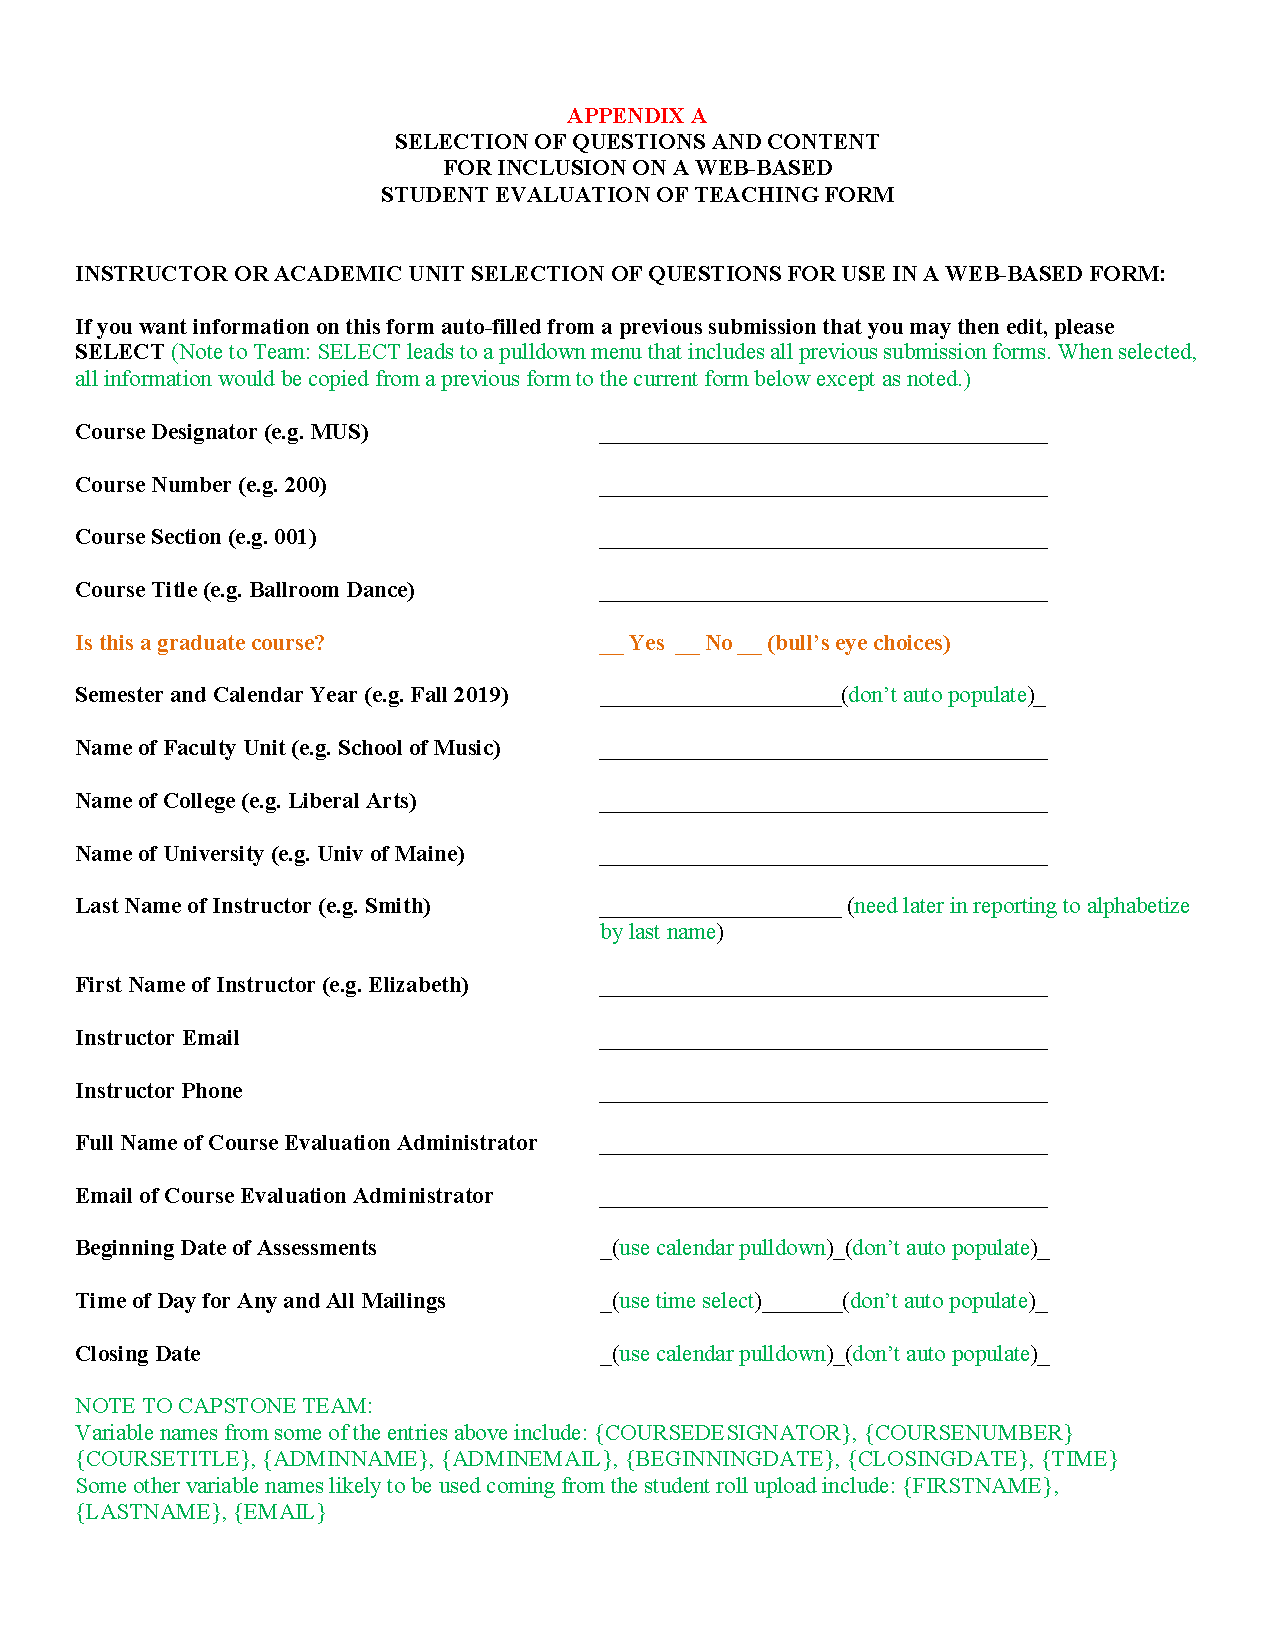
\includepdf[scale=0.85,pages=1,pagecommand=\section{Example Question Selection Form}]{images/question_appendix.pdf}
\includepdf[scale=0.85,pages=2-]{images/question_appendix.pdf}

\newpage

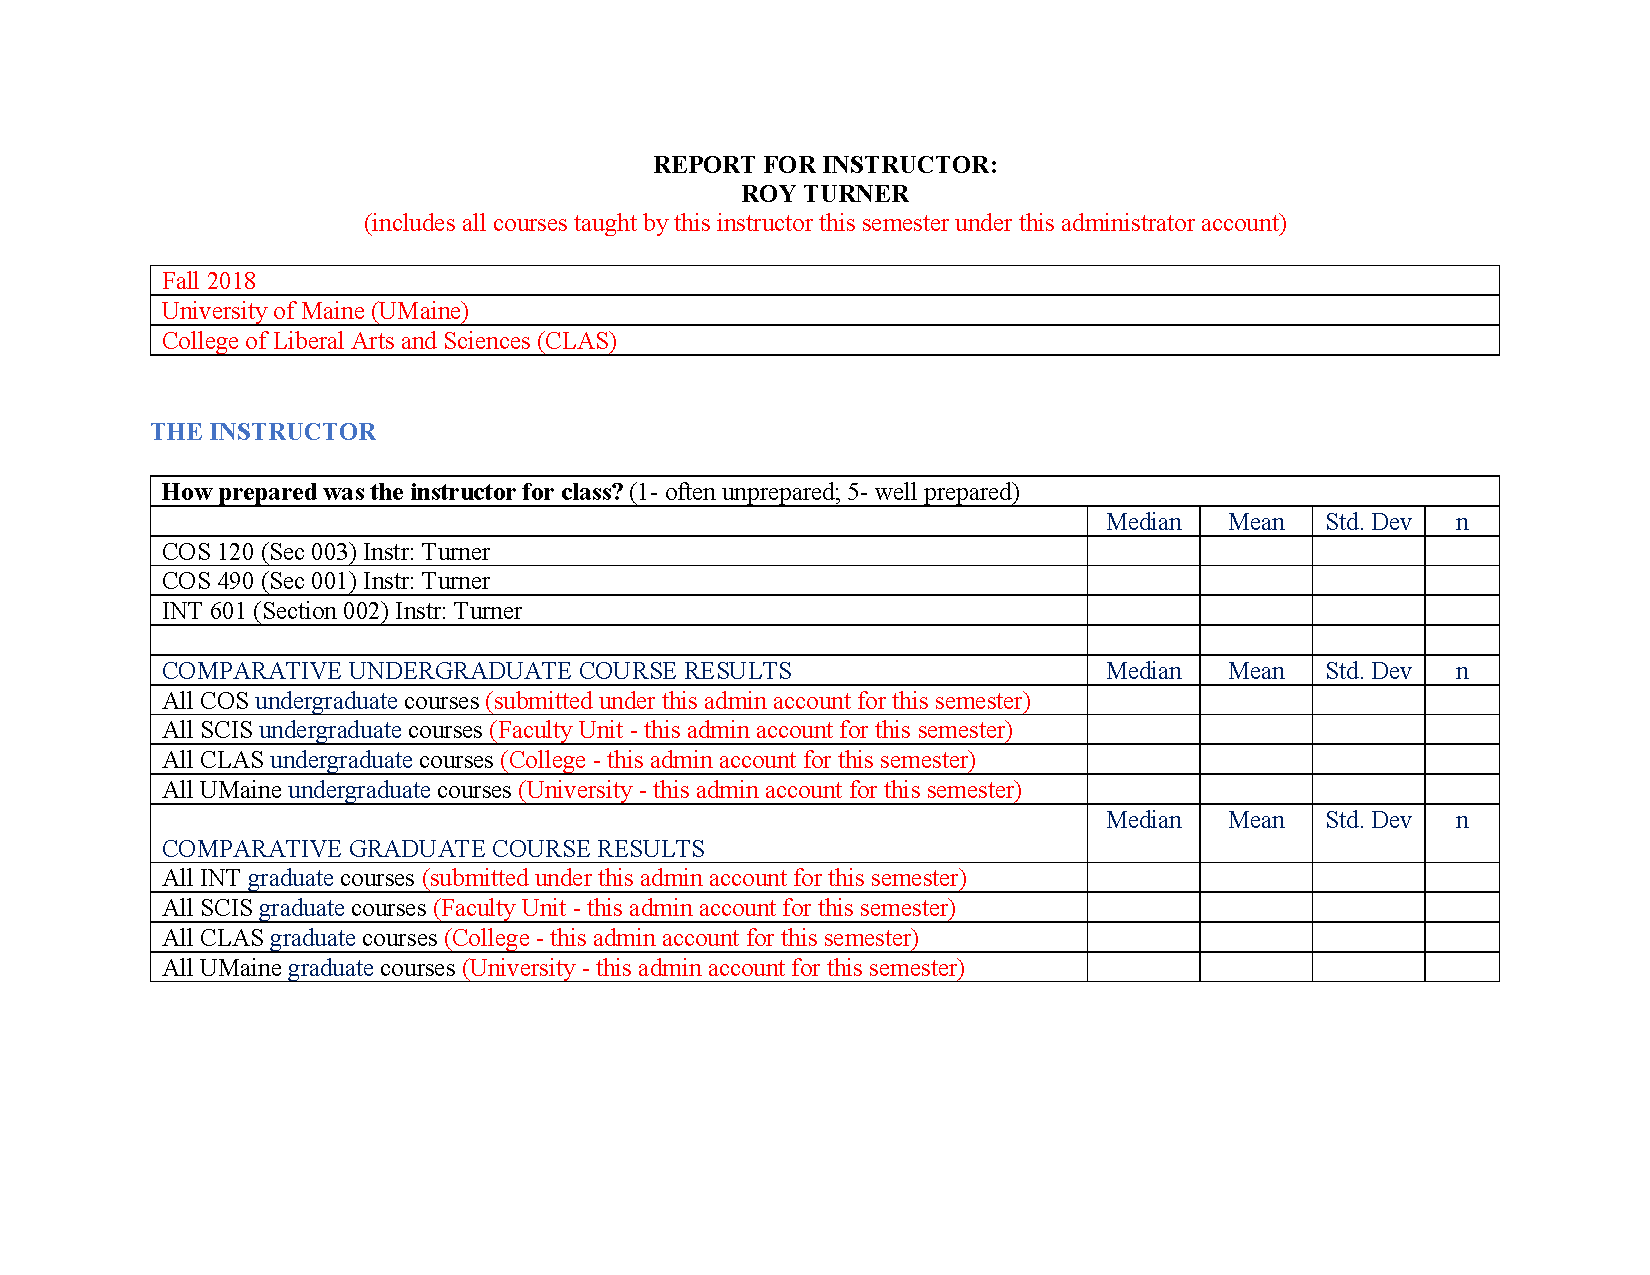
\includepdf[scale=0.92,pages=1,pagecommand=\section{Example Results Display}]{images/results_appendix.pdf}
\includepdf[scale=0.92,pages=2-]{images/results_appendix.pdf}
\end{document}
